\documentclass[14pt, aspectratio=169]{beamer}
\usetheme{copenhagen}
\usecolortheme{seahorse}

\setbeamertemplate{navigation symbols}{}
\setbeamertemplate{headline}{} 
\setbeamertemplate{footline}{} 
\setbeamercovered{transparent} 

\usepackage{amsmath, amsfonts, amssymb, enumerate, tfrupee, xcolor, lipsum, minted, algorithm, algpseudocode, algorithmicx, float, hyperref, booktabs, graphicx, array}

\title{A Classification Based approach for predicting Smartphone Price Categories}
\author{\textbf{Sayan Das} - B2430035 \and \textbf{Raihan Uddin} - B2430070}
\date{\today}

\begin{document}
\maketitle

\begin{frame}{Outline}
  \tableofcontents
\end{frame}



\section{Introduction}
\begin{frame}{}
  \Huge
  \centering
  \textbf{Introduction}
  \normalsize
\end{frame}
\begin{frame}{Background}
    \begin{itemize}
      \item The smartphone industry experiences continuous technological innovations, with manufacturers introducing advanced features.
      \item Multiple global players, such as Apple, Samsung, and Xiaomi, vie for market share, leading to frequent product launches and \textbf{pricing battles}.
      \item Consumers demand \textbf{value for money}, with preferences shifting toward devices offering high performance at competitive prices.
  \end{itemize}
\end{frame}
\begin{frame}{Motivation}
  We hope our model will help:
  \vspace{1.25em}
  \begin{itemize}
	\setlength\itemsep{1em}
    \item<1-> Simplify pricing strategies for \textbf{manufacturers}
    \item<2-> Increase pricing transparency for \textbf{consumers}
  \end{itemize}
\end{frame}
\begin{frame}{Objectives}
  \begin{itemize}
	\setlength\itemsep{0.75em}
    \item<1-> Develop a Robust Classification Model
    \item<2-> Determine the most influential factors behind smartphone pricing
    \item<3-> Compare algorithm performances
    \item<4-> Practical Applicability
    \item<5-> Methodological Contribution
  \end{itemize}
\end{frame}


\section{Dataset Description}
\begin{frame}{}
  \Huge
  \centering
  \textbf{Dataset Description}
  \normalsize
\end{frame}
\begin{frame}{Source}
  \begin{figure}[H]
    \centering
    
\includegraphics[width=0.3\textwidth]{kaggle.png}
  \end{figure}
  Link - \footnotesize \href{https://www.kaggle.com/datasets/iabhishekofficial/mobile-price-classification?select=train.csv}{https://www.kaggle.com/datasets/iabhishekofficial/smartphone-price-classification}\\
  \normalsize
  
  The dataset is publicly available and contains \textbf{2000 smartphone entries} with \textbf{19 feature variables} and \textbf{1 target variable} representing \texttt{price\_range}.
\end{frame}
\begin{frame}{Features}
  \vspace{-0.25em}
  \scriptsize
  \begin{table}[H]
    \begin{tabular}{lll}
      \toprule
      \textbf{Feature Name}   & \textbf{Description}  & \textbf{Type}  \\
      \toprule
      \texttt{battery\_power} & battery capacity in mAh   & Numerical  \\
      \texttt{clock\_speed}   & speed at which processor executes instructions & Numerical \\
      \texttt{fc}             & front Camera Megapixels & Numerical \\
      \texttt{pc}             & primary Camera Megapixels & Numerical \\
      \texttt{int\_memory}    & internal Memory capacity & Numerical \\
      \texttt{m\_dep}         & smartphone Depth in cm & Numerical \\
      \texttt{mobile\_wt}     & weight of the smartphone & Numerical \\
      \texttt{n\_cores}       & number of cores in processor & Numerical \\
      \texttt{px\_height}     & pixel Resolution Height & Numerical \\
      \texttt{px\_width}      & pixel Resolution Width & Numerical \\
      \texttt{ram}            & RAM in MB & Numerical \\
      \texttt{sc\_h}          & screen Height in cm & Numerical \\
      \texttt{sc\_w}          & screen Width in cm & Numerical \\
      \texttt{talk\_time}     & longest time that a single battery charge will last over a call & Numerical \\
      \texttt{blue}           & has bluetooth or not  & Categorical   \\
      \texttt{dual\_sim}      & has dual sim support or not & Categorical \\
      \texttt{four\_g}        & has 4G or not & Categorical \\
      \texttt{three\_g}       & has 3G or not & Categorical \\
      \texttt{wifi}           & has wifi or not & Categorical \\
      \texttt{touch\_screen}  & has touch screen or not & Categorical \\
      \bottomrule
    \end{tabular}
  \end{table}
\end{frame}

\begin{frame}{Target Variable}
  \begin{itemize}
  \setlength\itemsep{0.5em}
  \item The target variable \texttt{price\_range} is \textbf{categorical} with \textbf{4 classes}.
  \begin{itemize}
  \setlength\itemsep{0.25em} \small
      \item \texttt{0} - Low Cost - \textbf{Budget} Smartphones
      \item \texttt{1} - Medium Cost - \textbf{Mid-Range} Smartphones
      \item \texttt{2} - High Cost - \textbf{High-End} Smartphones
      \item \texttt{3} - Very High Cost - \textbf{Flagship} Smartphones 
    \end{itemize}
    \normalsize
  \end{itemize}
\end{frame}

\section{Data Preprocessing}
\begin{frame}{}
  \Huge
  \centering
  \textbf{Data Preprocessing}
  \normalsize
\end{frame}

\begin{frame}[allowframebreaks]{Data Cleaning - Handling Missing Values}
  \begin{figure}[H]
    \centering
    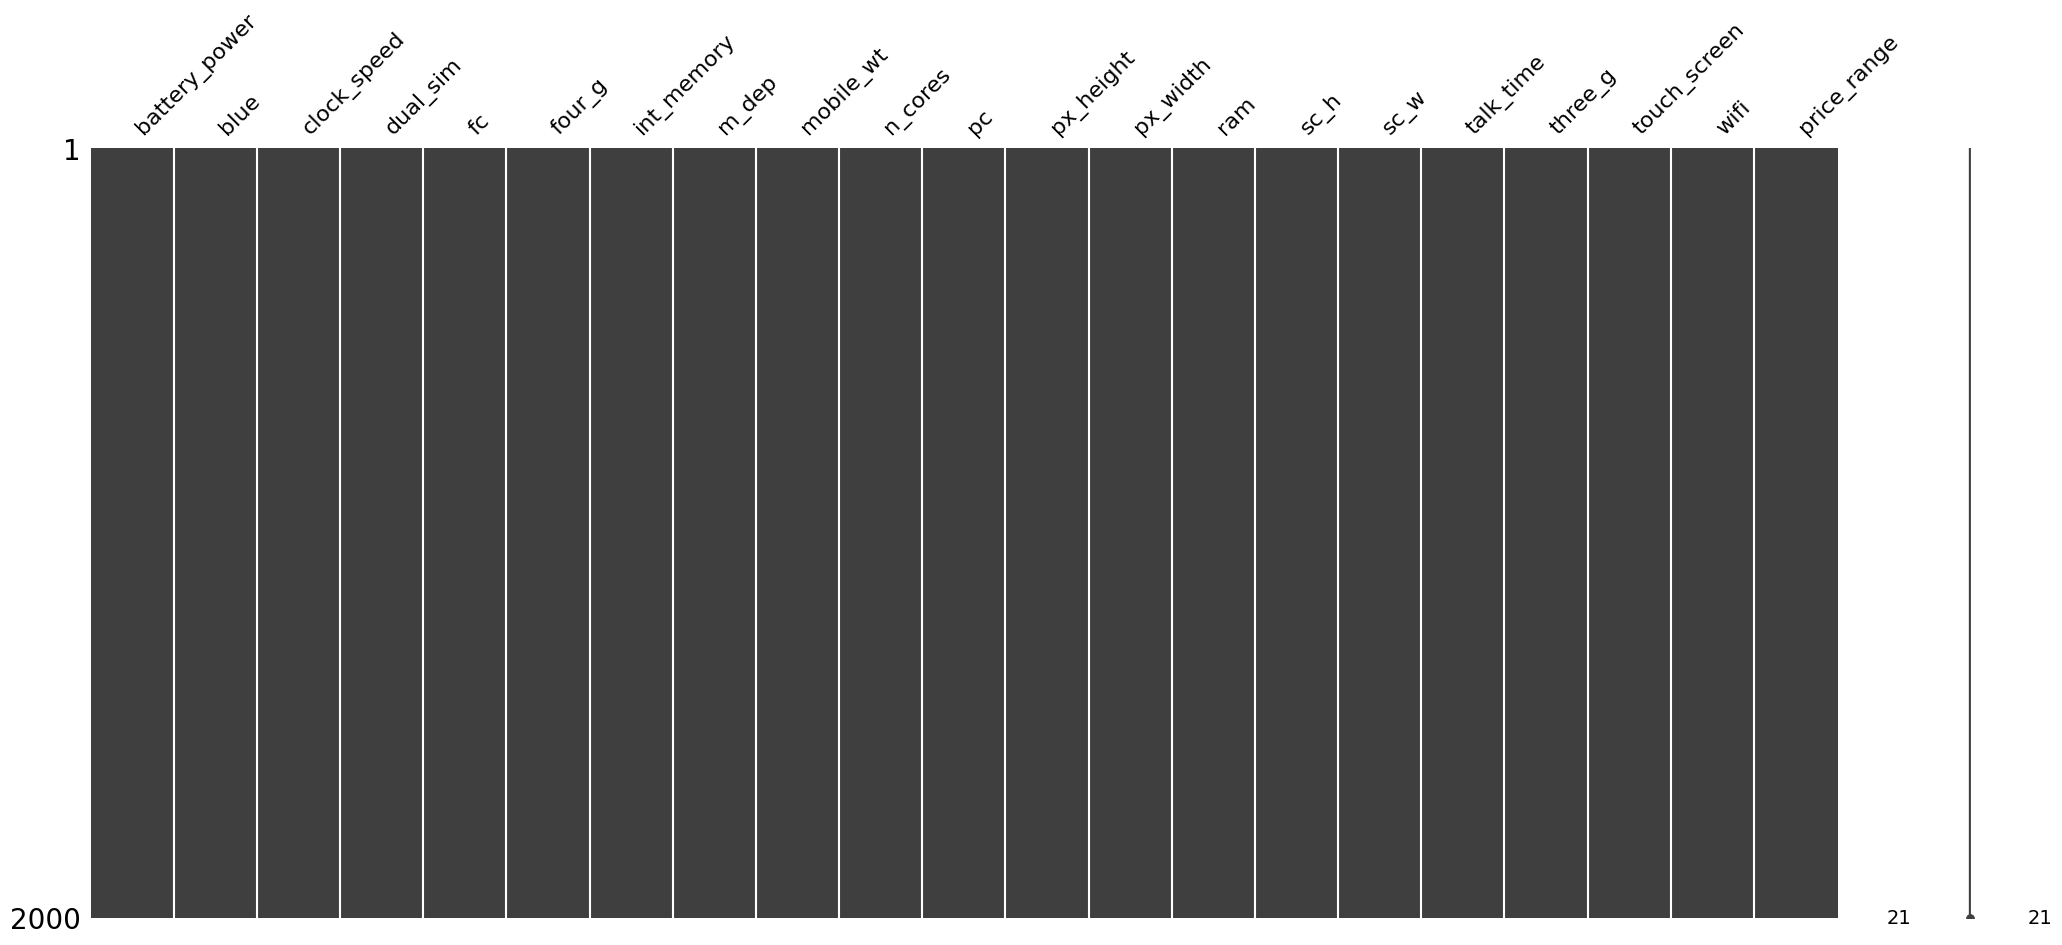
\includegraphics[height=0.3\textwidth]{missing_val.png}
  \end{figure}
  \begin{minipage}{0.475\textwidth}
    \begin{block}{}
      \textbf{Significance:} \small
      Machine learning models often require complete data to function correctly. Missing values can lead to errors.
    \end{block}
  \end{minipage}
  \hfill
  \begin{minipage}{0.475\textwidth}
    \begin{block}{}
      \textbf{Observation:} \small
      There are no missing values in the dataset.
    \end{block}
  \end{minipage}
\end{frame}

\begin{frame}[containsverbatim]{Data Cleaning - Handling Duplicate Values}
  \begin{minted}{python}
    df.duplicated().sum()
  \end{minted}
  \vspace{1em}
  \begin{minted}{python}
    np.int64(0)
  \end{minted}
  $ $\\
  \begin{minipage}{0.8\textwidth}
    \begin{block}{}
      \textbf{Significance:} \small
      Duplicate entries can distort the true representation of the data, leading to \textbf{bias}.
    \end{block}
    \begin{block}{}
      \textbf{Observation:} \small
      There are no duplicate values in the dataset.
    \end{block}
  \end{minipage}
\end{frame}

\begin{frame}[allowframebreaks, containsverbatim]{Data Cleaning - Handling Invalid Values}
  \begin{minted}{python}
negative_counts = df.apply(lambda x: (x < 0).sum())
print(negative_counts)
  \end{minted}
  \begin{minipage}{0.2\textwidth}
    
  \tiny
  \vspace{0.3em}
  \begin{minted}{python}
  battery_power    0
  blue             0
  clock_speed      0
  dual_sim         0
  fc               0
  four_g           0
  int_memory       0
  m_dep            0
  mobile_wt        0
  n_cores          0
  pc               0
  px_height        0
  px_width         0
  ram              0
  sc_h             0
  sc_w             0
  talk_time        0
  three_g          0
  touch_screen     0
  wifi             0
  price_range      0
  dtype: int64

  \end{minted}
  \normalsize
\end{minipage}
\hfill
\begin{minipage}{0.6\textwidth}
  \begin{block}{}
    \textbf{Significance:} \small
    None of the features can have negative values.
  \end{block}
  \begin{block}{}
    \textbf{Observation:} \small
    There are no negative values in the dataset.
  \end{block}
  
\end{minipage}

  \begin{minted}{python}
zero_counts = df.apply(lambda x: (x == 0).sum())
print(zero_counts)
  \end{minted}
  \begin{minipage}{0.2\textwidth}
    
  \tiny
  \vspace{0.3em}
  \begin{minted}{python}
battery_power       0
blue             1010
clock_speed         0
dual_sim          981
fc                474
four_g            957
int_memory          0
m_dep               0
mobile_wt           0
n_cores             0
pc                101
px_height           2
px_width            0
ram                 0
sc_h                0
sc_w              180
talk_time           0
three_g           477
touch_screen      994
wifi              986
price_range       500
dtype: int64

  \end{minted}
  \normalsize
\end{minipage}
\hfill
\begin{minipage}{0.6\textwidth}
  \small
  \begin{block}{}
    \textbf{Significance:} \small
    Most of the numerical features can not be zero except \texttt{fc} and \texttt{pc}. These two being zero means the phone does not have a front or primary camera.
  \end{block}
  \begin{block}{}
    \textbf{Observation:} \small
    \texttt{px\_height} and \texttt{sc\_w} are have 2 and 180 zero values respectively.
  \end{block}
  \begin{block}{}
    \textbf{Action:} \small
    We replaced these zero values with the mean of the respective features.
  \end{block}
\end{minipage}
\small
\begin{minted}{python}
to_replace_with_mean = ['sc_w', 'px_height']

for feature in to_replace_with_mean:
  df[feature] = df[feature].replace(0, df[feature].mean())
\end{minted}
  \normalsize
\end{frame}

\begin{frame}[allowframebreaks]{Data Cleaning - Outlier Handling}
  \begin{minipage}{0.8\textwidth}
    \begin{block}{}
      \textbf{Significance:} \small
      \begin{itemize}
        \item Outliers can distort the true representation of data.
        \item Machine learning models can be sensitive to outliers.
      \end{itemize}
    \end{block}
  \end{minipage}
  \begin{figure}[H]
    \centering
    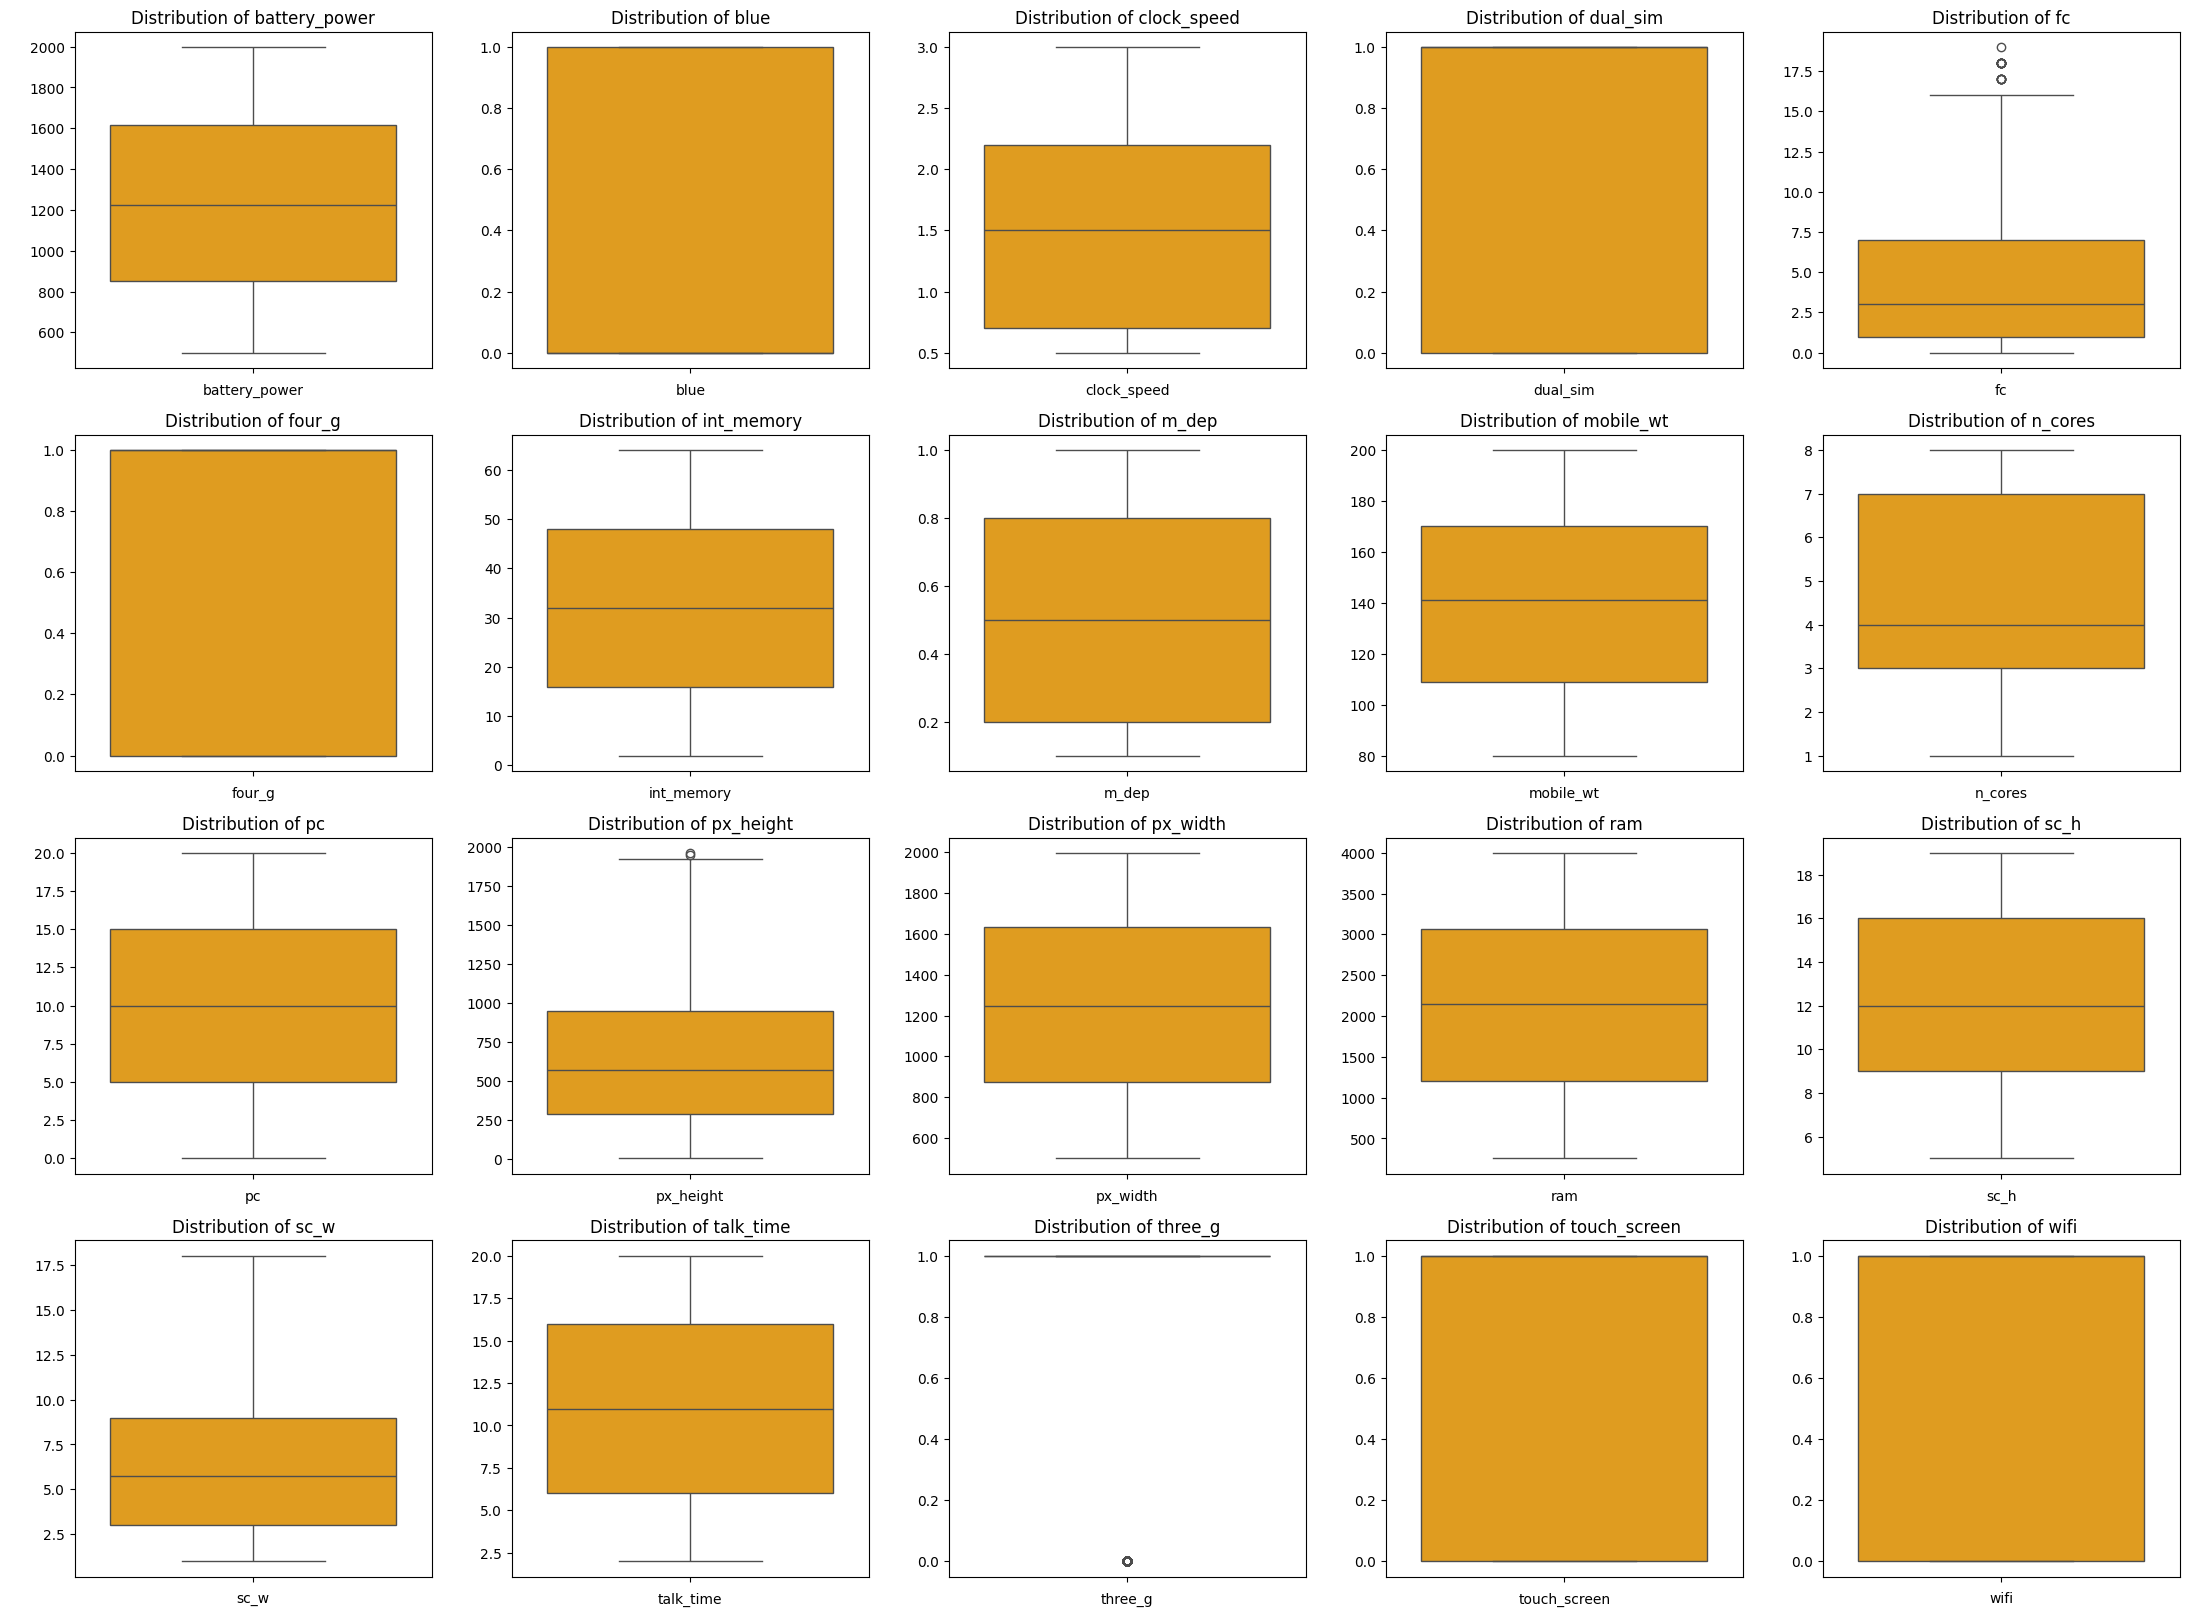
\includegraphics[width=0.75\textwidth]{../report/box_plots_before.png}
  \end{figure}
\end{frame}

\begin{frame}{Data Cleaning - Outlier Handling (cont.)}
  \begin{minipage}{0.8\textwidth}
    \begin{block}{}
      \textbf{Observation:} \small
      The box plots revealed outliers in two features, \texttt{fc} and \texttt{px\_height}.
    \end{block}
  \end{minipage}
  \begin{minipage}{0.8\textwidth}
    \begin{block}{}
      \textbf{Action:} \small
      To identify these outliers, we will use the IQR (Interquartile Range) method and remove extreme values.
    \end{block}
  \end{minipage}
  \footnotesize
  \[
  \text{IQR} = Q3 - Q1
  \]
  Once the IQR is calculated, outliers are identified using the following bounds:
  \[
  \text{Lower Bound} = Q1 - 1.5 \times \text{IQR} \quad \quad \quad \text{Upper Bound} = Q3 + 1.5 \times \text{IQR}
  \]
  Any data point that falls below the lower bound or above the upper bound is considered an outlier.
  \normalsize
\end{frame}

\begin{frame}[containsverbatim]{Data Cleaning - Outlier Handling (cont.)}
\footnotesize
\begin{minted}{python}
def remove_outliers_iqr(data, column):
  Q1 = data[column].quantile(0.25)
  Q3 = data[column].quantile(0.75)
  IQR = Q3 - Q1

  lower_bound = Q1 - 1.5 * IQR
  upper_bound = Q3 + 1.5 * IQR

  filtered_data = data[(data[column] >= lower_bound) &
                       (data[column] <= upper_bound)]
  return filtered_data

df = remove_outliers_iqr(df, 'fc')
df = remove_outliers_iqr(df, 'px_height')
\end{minted}

\end{frame}

\begin{frame}[containsverbatim]{Data Cleaning - Outlier Handling (cont.)}
  \begin{figure}[H]
    \centering
    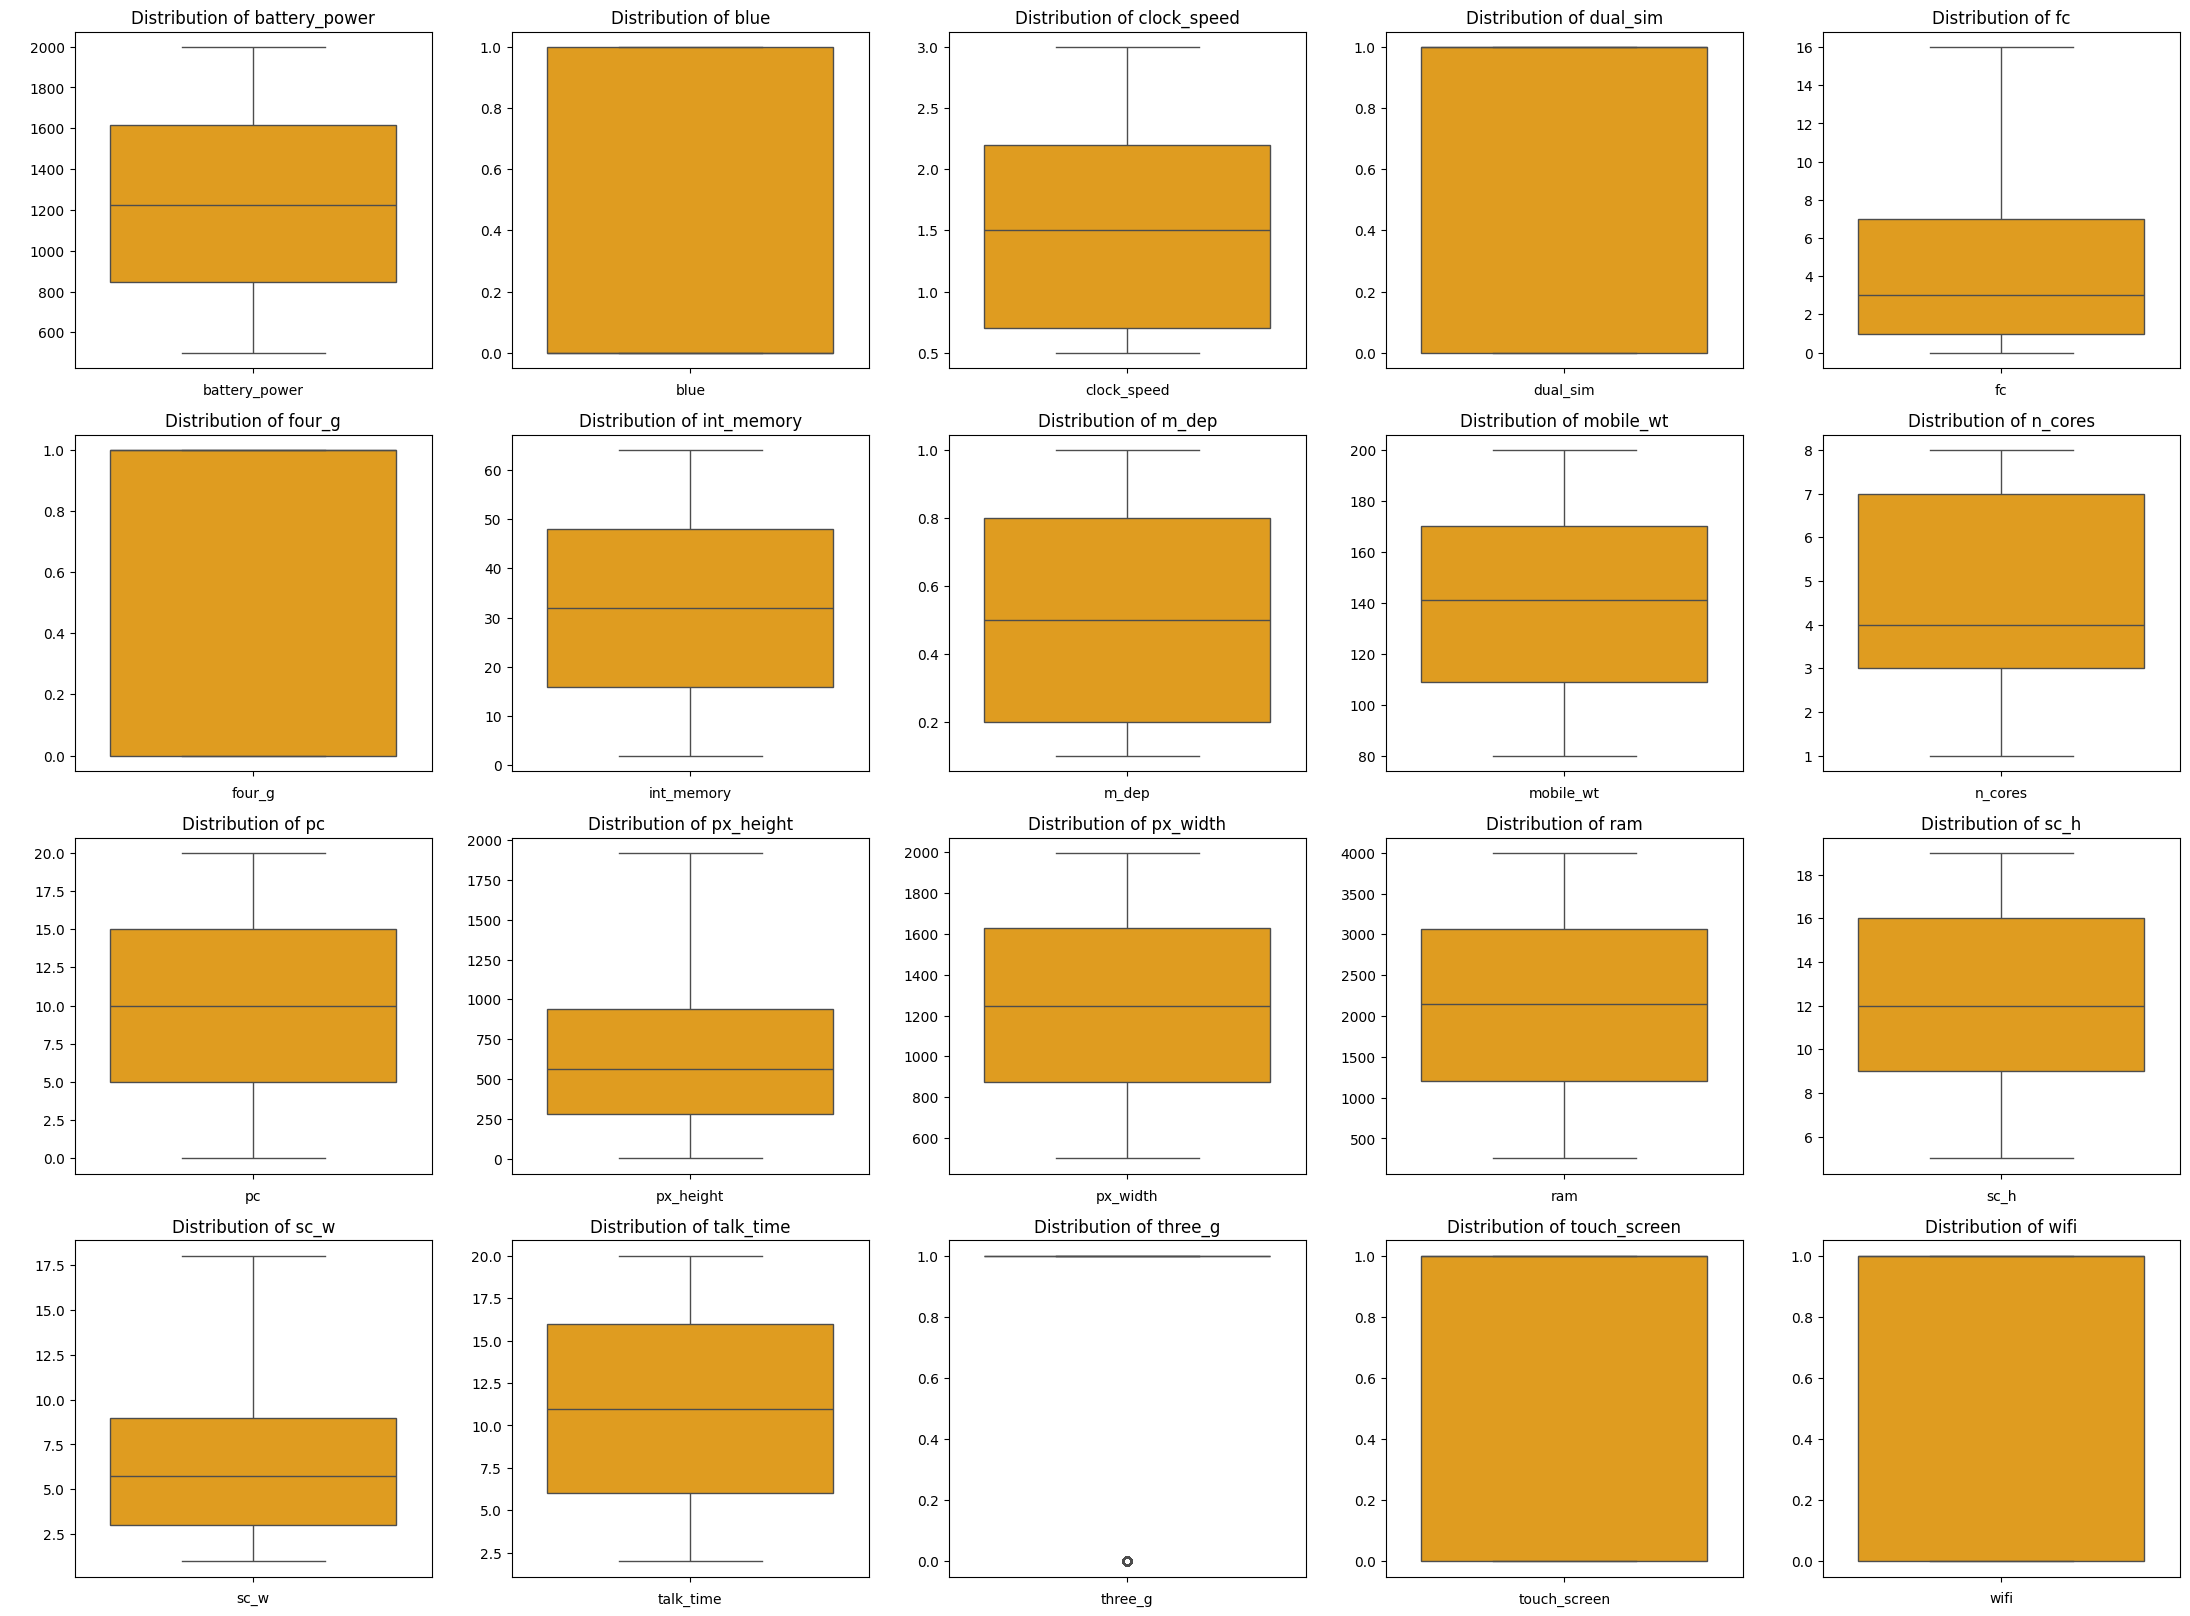
\includegraphics[width=0.7\textwidth]{../report/box_plots_after.png}
  \end{figure}
\end{frame}
\begin{frame}{Data Cleaning - Checking for Class Imbalance}
  \begin{figure}[H]
    \centering
    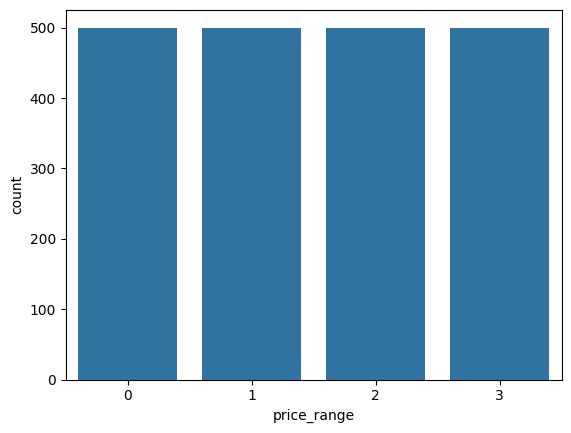
\includegraphics[height=0.3\textwidth]{../report/imbalance_check.png}
  \end{figure}
  \begin{minipage}{0.475\textwidth}
    \begin{block}{}
      \textbf{Significance:} \small
      Imbalanced dataset makes the model biased towards the majority class.
    \end{block}
  \end{minipage}
  \hfill
  \begin{minipage}{0.475\textwidth}
    \begin{block}{}
      \textbf{Observation:} \small
      There are no class imbalance in the dataset.
    \end{block}
  \end{minipage}
\end{frame}


\begin{frame}[allowframebreaks, containsverbatim]{Data Cleaning - Correlation Analysis}
  \begin{minipage}{0.3\textwidth}    
    \begin{block}{}
      \textbf{Significance:} \small
      Correlation analysis helps identify relationships between features. It can help in feature engineering.
    \end{block}
    \normalsize
  \end{minipage}
  \hfill
  \begin{minipage}{0.6\textwidth}
    \begin{figure}[H]
      \centering
      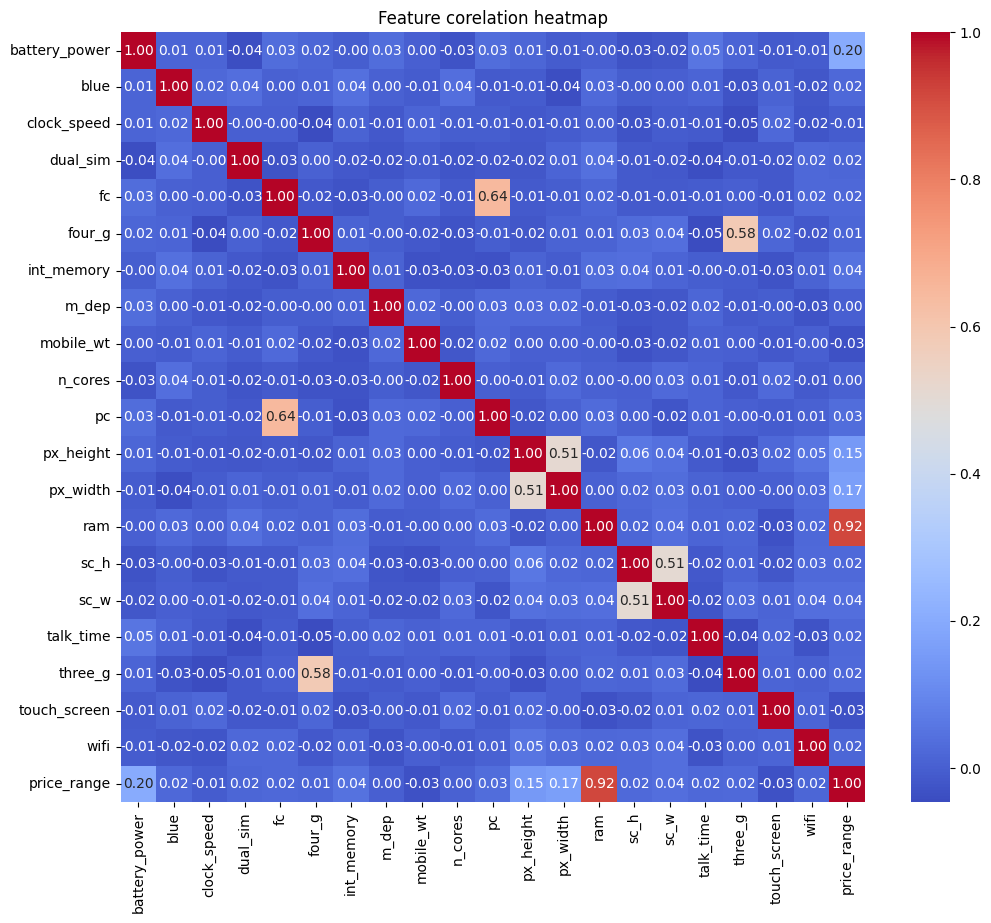
\includegraphics[width=0.98\textwidth]{../report/corr_viz.png}
    \end{figure}
  \end{minipage}

  \begin{block}{}
    \textbf{Observation:} \small
    \begin{enumerate}
      \setlength\itemsep{.05em}
      \item{\textbf{ram and price\_range :}} Higher RAM capacity leads to higher price range.
      \item{\textbf{three\_g and four\_g :}} A high correlation here suggests that devices with 4G almost always support 3G, making one of these features redundant.
      \item{\textbf{fc and pc :}} These features are correlated, as better primary cameras often accompany better front cameras.
      \item{\textbf{px\_height and px\_width :}} These are components of screen resolution and are naturally correlated.
      \item{\textbf{sc\_h and sc\_w :}} These are also naturally correlated.
    \end{enumerate}
  \end{block}
  
  \begin{block}{}
    \textbf{Action:} \small
    \begin{enumerate}
      \setlength\itemsep{.05em}
      \item{\textbf{three\_g and four\_g :}} \texttt{three\_g} was removed from the dataset.
      \item{\textbf{fc and pc :}} \texttt{fc} was removed from the dataset.
      \item{\textbf{px\_height and px\_width :}} They were combined to form a new feature \texttt{px\_area = px\_height * px\_width}.
      \item{\textbf{sc\_h and sc\_w :}} They were combined to form a new feature \texttt{screen\_area = sc\_h * sc\_w}.
    \end{enumerate}
  \end{block}

  \begin{minipage}{0.6\textwidth}
    \begin{figure}[H]
      \centering
      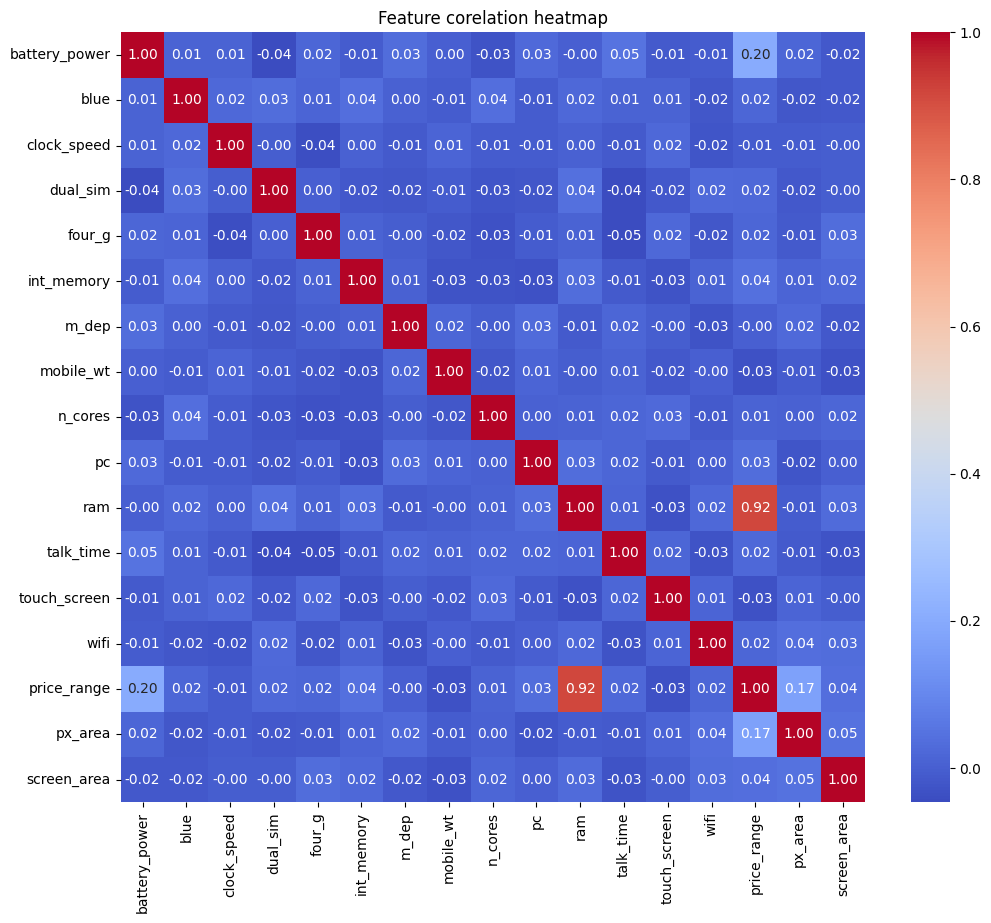
\includegraphics[width=0.98\textwidth]{../report/corr_viz_after_fe.png}
    \end{figure}
  \end{minipage}
  \hfill
  \begin{minipage}{0.3\textwidth} \small
    Correlation Matrix after feature engineering
    \normalsize
  \end{minipage}
\end{frame}

\begin{frame}[allowframebreaks, containsverbatim]{Feature Selection}
  \begin{block}{}
    \textbf{Significance:} \small
    By selecting the most relevant features, the model can focus on the \textbf{most important} information. Moreover, including irrelevant or redundant features can cause the model to \textbf{overfit} the training data. Also, fewer features mean \textbf{less data to process}.
  \end{block}
  \begin{block}{}
    \textbf{Action:} \small
    In our project, we used the ANOVA F-test (Analysis of Variance) method to evaluate each feature's relationship with the target variable, price\_range, and select features that are statistically significant. The threshold for selection is a p-value of less than $0.1$ i.e. a $90\%$ confidence level.
  \end{block}
\footnotesize
  \begin{minted}{python}
y = df.pop('price_range')
X = df
feature_selector = SelectKBest(f_classif, k='all')  
X_selected = feature_selector.fit_transform(X, y)
p_values = feature_selector.pvalues_
f_scores = feature_selector.scores_

selected_features = X.columns[p_values < 0.1]
  \end{minted}
  \normalsize
  \begin{block}{}
    \textbf{Outcome:} \small
    The selected features are: \\
    \texttt{'battery\_power', 'int\_memory', 'mobile\_wt', 'n\_cores', 'ram', 'px\_area', 'screen\_area'}
  \end{block}
\end{frame}
\begin{frame}[allowframebreaks]{Normalizing Features}
  \begin{block}{}
    \textbf{Significance:} \small
    Normalizing features ensures that all features contribute equally to the model training process and prevents any feature from dominating the others.
  \end{block}
  \begin{block}{}
    \textbf{Action:} \small
    We used the \texttt{PowerTransformer} from \texttt{sklearn.preprocessing} to normalize the features \texttt{px\_area} and \texttt{screen\_area}.
  \end{block}
  \begin{block}{}
    \textbf{Outcome:} \small
    The features \texttt{px\_area} and \texttt{screen\_area} were successfully normalized, resulting in a more balanced dataset for model training.
  \end{block}
\end{frame}

\begin{frame}[allowframebreaks]{Train-Test Split}
  \begin{block}{}
    \textbf{Significance:} \small
    Splitting the dataset into training and testing sets allows us to evaluate model performance and ensure that the model generalizes well to unseen data.
  \end{block}
  \begin{block}{}
    \textbf{Action:} \small
    We used \texttt{train\_test\_split} from \texttt{sklearn.model\_selection} to split the dataset into 80\% training and 20\% testing sets.
  \end{block}
  \begin{block}{}
    \textbf{Outcome:} \small
    The train-test split resulted in 1584 samples with 7 features for training and 396 samples with 7 features for testing, with corresponding target arrays of 1584 and 396 elements, respectively.
  \end{block}
\end{frame}

\begin{frame}[allowframebreaks]{Scaling}
  \begin{block}{}
    \textbf{Significance:} \small
    Scaling ensures that all feature values are normalized, which improves the performance and convergence of many machine learning algorithms.
  \end{block}
  \begin{block}{}
    \textbf{Action:} \small
    We used the \texttt{StandardScaler} from \texttt{sklearn.preprocessing} to scale the feature values.
  \end{block}
  \begin{block}{}
    \textbf{Outcome:} \small
    The dataset was successfully scaled, resulting in normalized feature values that contribute equally to the model training process.
  \end{block}
\end{frame}
\section{Acknowledgement}
\begin{frame}{Acknowledgement}
\end{frame}

\section{References}
\begin{frame}{References}
\end{frame}

\begin{frame}{}
  \Huge
  \centering
  \textbf{Thank You!}
\end{frame}

\end{document}
